\subsection{Manipulationsknoten}

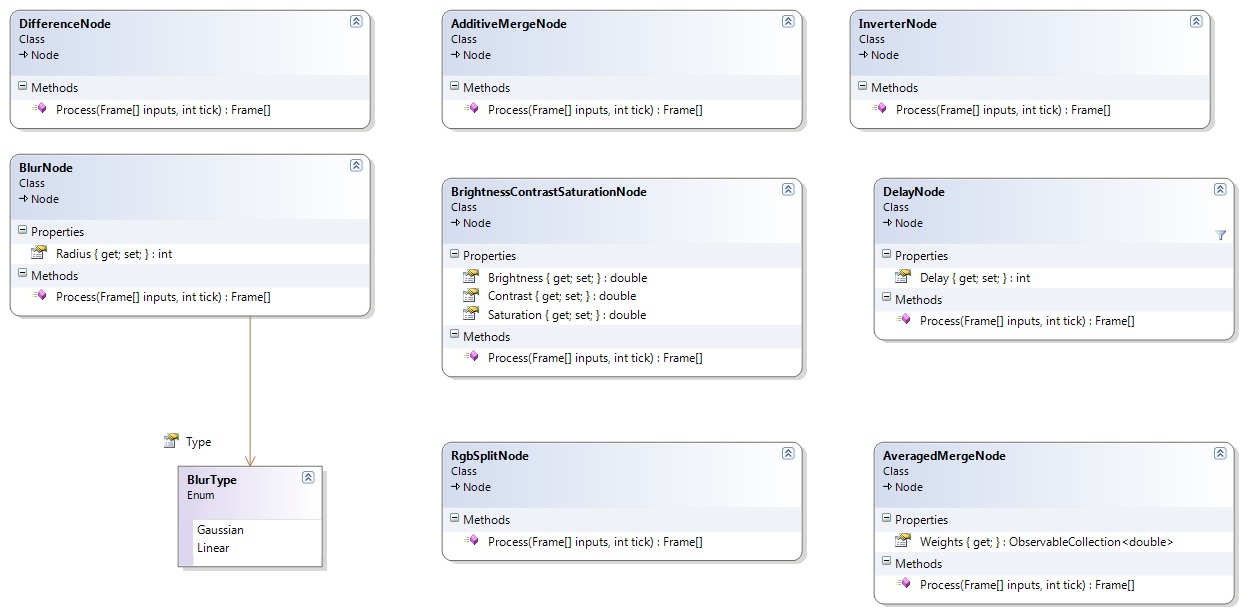
\includegraphics[width=\textwidth]{YuvKA.Pipeline/manipulationnodes.png}
Diese Klassen sind für die Manipulation der Videos innerhalb der Pipeline zuständig. Die einzelnen Knoten sowie deren Implementation werden im Folgenden erläutert. All diese Knoten erben von der abstrakten Klasse \name{Node}.

\subsubsection{YuvKA.Pipeline.InverterNode}
\begin{verbatim}
public class InverterNode : Node
\end{verbatim}

\paragraph{Beschreibung}~\\
Die Klasse \name{InverterNode} invertiert die Farben des \name{Frame}s.

\paragraph{Typmember}
\begin{itemize}

\method{ProcessFrame}
	\begin{verbatim}
	public override Frame[] ProcessFrame(Frame[] inputs, int tick)
	\end{verbatim}
	Invertiert die Farbe der einzelnen Pixel des \name{Frame}s. Dafür wird das Komplement von jedem der drei Farbkanäle eines Pixels gebildet.

\end{itemize}


\subsubsection{YuvKA.Pipeline.BlurNode}

\begin{verbatim}
[DataContract]
public class BlurNode : Node
\end{verbatim}

\paragraph{Beschreibung}~\\
Die Klasse \name{BlurNode} modelliert die Weichzeichnung der \name{Frame}s des Videos.

\paragraph{Typmember}
\begin{itemize}

\property{Type}
	\begin{verbatim}
	[DataMember]
	public BlurType Type { get; set; }
	\end{verbatim}
	Ruft die Art der Weichzeichnung ab oder legt sie fest. Standardmäßig werden gaußsches und lineares Weichzeichnen unterstützt.
	
\property{Radius}
	\begin{verbatim}
	[DataMember]
	[Range(0.0, double.PositiveInfinity)]
	public int Radius { get; set; }
	\end{verbatim}
	Ruft den Weichzeichnungsradius ab oder legt diesen fest. Dieser Wert ist maßgeblich für das Ausmaß der Weichzeichnung.

\method{ProcessFrame}
	\begin{verbatim}
	public override Frame[] ProcessFrame(Frame[] inputs, int tick)
	\end{verbatim}
	Zeichnet den übergebenen \name{Frame} weich. Die genaue Art der Weichzeichnung wird hierbei durch \name{Type} festgelegt. Die standardmäßig unterstützten Arten sind:
	\begin{description}
		\item[Lineares Weichzeichnen]~\\
			Beim linearen Weichzeichnen wird der neue Wert eines Pixels dadurch berechnet, dass die alten Werte aller umliegenden Pixel innerhalb einer Box mit Höhe und Breite (2 * \name{Radius}) + 1 gemittelt werden. Über den \name{Frame}rand hinaus benötigte Pixel werden durch den Pixel, der dem gesuchten Pixel am nächsten ist, simuliert. ~\\~\\
			PseudoCode:
			\begin{verbatim}
				Frame newFrame = new Frame(inputs[0])
				for (int x = 0; x < inputs[0].Size.X; x++)
				  for (int y = 0; y < inputs[0].Size.Y; y++)
				    newFrame(x, y) = 0
				    for (xi = x - Radius; xi <= x + Radius; xi++)
				      for (yi = y - Radius; yi <= y + Radius; yi++)
				        newFrame(x, y) += (1 / (Radius * Radius))
				                           * inputs[0](x, y)
				return newFrame
				
			\end{verbatim}
		\item[Gaußsches Weichzeichnen]~\\
			Beim Gaußschen Weichzeichnen wird der neue Wert eines Pixels durch eine gewichtete Mittelung der umliegenden Pixel berechnet. Die Gewichtung der umliegenden Pixel wird hierbei durch folgende gaußsche Funktion definiert:\\
			\[
			G(x,y) = \frac{1}{\sqrt{2\pi\sigma^2}}e^{-\frac{x^2}{2\sigma^2}}
			\]
			Wobei $\sigma$ der \name{Radius} ist.\\
			 Über den \name{Frame}rand hinaus benötigte Pixel werden durch den Pixel, der dem gesuchten Pixel am nächsten ist, simuliert.~\\~\\
			PseudoCode:
			\begin{verbatim}
				Frame newFrame = new Frame(inputs[0])
				for (int x = 0, x < inputs[0].size.x, x++)
				  for (int y = 0, y < inputs[0].size.y, y++)
				    newFrame.Data[x][y] = 0
				    for (int xi = x - (3 * Radius); xi < x + (3 * Radius;, xi++)
				      for (int yi = y - (3 * Radius); yi < y + (3 * Radius); yi++)
				        newFrame.Data[x][y] += G(xi - x, yi - y) * inputs[0].Data[x][y]
				return newFrame
				
			\end{verbatim}
	\end{description}
	
\end{itemize}


\subsubsection{YuvKA.Pipeline.BrightnessContrastSaturationNode}

\begin{verbatim}
[DataContract]
public class BrightnessContrastSaturationNode : Node
\end{verbatim}

\paragraph{Beschreibung}~\\
Diese Klasse \name{BrightnessContrastSaturationNode} ändert die Helligkeit, den Kontrast und/oder die Farbsättigung des \name{Frame}s.

\begin{itemize}

\property{Brightness}
	\begin{verbatim}
	[DataMember]
	[Range(-1.0, 1.0)]
	public double Brightness
	\end{verbatim}
	Ruft den Helligkeitswert, zu dem dieses \name{Frame} gesetzt werden soll, ab oder legt ihn fest. Der Wert muss zwischen -1.0 und 1.0 liegen.
	
\property{Contrast}
	\begin{verbatim}
	[DataMember]
	[Range(-1.0, 1.0)]
	public double Contrast
	\end{verbatim}
	Ruft den Kontrastwert, zu dem dieses \name{Frame} gesetzt werden soll, ab oder legt ihn fest. Der Wert muss zwischen -1.0 und 1.0 liegen.
	
\property{Saturation}
	\begin{verbatim}
	[DataMember]
	[Range(-1.0, 1.0)]
	public double Saturation
	\end{verbatim}
	Ruft den Farbsättigungswert, zu dem dieses \name{Frame} gesetzt werden soll, ab oder legt ihn fest. Der Wert muss zwischen -1.0 und 1.0 liegen.

\method{ProcessFrame}
	\begin{verbatim}
	public override Frame[] ProcessFrame(Frame[] inputs, int tick)
	\end{verbatim}
	Die Methode \name{ProcessFrame} setzt die Helligkeit, den Kontrast und die Farbsättigung des \name{Frame}s auf die gegebenen Werte. Dafür werden die Farbkanäle jedes Pixels aus dem RGB-Raum in den HSV-Raum umgerechnet, die Änderungen vorgenommen und anschließend wieder nach RGB konvertiert, wie in folgenden beiden Algorithmen zu sehen ist:
	\floatname{algorithm}{Algorithmus}
	\begin{algorithm}[H]
	\caption{RGB nach HSV Konvertierung}
		\begin{algorithmic}[1]
		\REQUIRE $ R, G, B \in [0, 1] $
		\STATE $ MAX \gets \text{max}(R, G, B) $
		\STATE $ MIN \gets \text{min}(R, G, B) $ 
		\vspace{5px}
		\STATE $
					H \gets
					\begin{cases}
						0^{\circ}, & \text{falls } MAX = MIN \Leftrightarrow R = G = B \\
						60^{\circ}\cdot(0 + \frac{G - B}{MAX - MIN}), & \text{falls } MAX = R \\
						60^{\circ}\cdot(2 + \frac{B - R}{MAX - MIN}), & \text{falls } MAX = G \\
						60^{\circ}\cdot(4 + \frac{R - G}{MAX - MIN}), & \text{falls } MAX = B
					\end{cases}
				$  
				\vspace{5px}
		\IF {$ H < 0^{\circ} $}
			\STATE $ H \gets H + 360^{\circ} $
		\ENDIF 
		\vspace{5px}
		\STATE $ 
					S \gets
					\begin{cases}
						0, & \text{falls } MAX = 0 \Leftrightarrow R = G = B = 0 \\
						\frac{MAX - MIN}{MAX}, & \text{sonst}
					\end{cases}
				$
		\vspace{5px}
		\STATE $ V \gets MAX $ 
		\ENSURE $ H \in [0^{\circ}, 360^{\circ}],\ S, V \in [0, 1] $
	\end{algorithmic}
	\end{algorithm}
	
	\begin{algorithm}[H]
	\caption{HSV nach RGB Konvertierung}
		\begin{algorithmic}[1]
			\REQUIRE $ H \in [0^{\circ}, 360^{\circ}],\ S, V \in [0, 1] $ \\
			\COMMENT{Es werden das Grundfarbenintervall h, der Wert innerhalb dieses Intervalls f in [0,1] und noch drei Hilfswerte bestimmt, die bereits die jeweiligen Streckenlängen enthalten, aber entsprechend auf die Komponenten R, G und B zu verteilen sind:}
			\STATE $ h \gets \lfloor\frac{H}{60^\circ}\rfloor $
			\STATE $ f \gets \frac{H}{60^{\circ}} - h $
			\STATE $ p \gets V \cdot (1 - S) $ 
			\STATE $ q \gets V \cdot (1 - S \cdot f) $
			\STATE $ t \gets V \cdot (1 - S \cdot (1 - f)) $
			\vspace{5px}
			\STATE $
						(R, G, B) \gets
						\begin{cases}
							(V, t, p), & \text{falls } h \in \{0, 6\} \\
							(q, V, p), & \text{falls } h = 1 \\
							(p, V, t), & \text{falls } h = 2 \\
							(p, q, V), & \text{falls } h = 3 \\
							(t, p, V), & \text{falls } h = 4 \\
							(V, p, q), & \text{falls } h = 5
						\end{cases}
					$
			\vspace{5px}
			\ENSURE $ R, G, B \in [0, 1] $ \\
			\COMMENT {Ist S = 0, dann ist die resultierende Farbe Neutralgrau, und die Formel vereinfacht sich zu R = G = B = V.}
		\end{algorithmic}
	\end{algorithm} 

	Nach der RGB - HSV Konvertierung können die S (Sättigung) und V (Helligkeit) Werte in den oben angegebenen Schranken modifiziert werden, um dann wieder nach RGB umgewandelt zu werden und in den neuen Pixeln geschrieben zu werden. \\
	Für den Kontrast ist lediglich der Abstand zwischen einem Farbkanal und 128 zu vergrößern, wie in der folgenden Formel zu sehen ist: \begin{eqnarray*}
   r = (r - 128) \cdot \text{\name{Contrast}} + 128 \\
	g = (g - 128) \cdot \text{\name{Contrast}} + 128 \\
	b = (b - 128) \cdot \text{\name{Contrast}} + 128
\end{eqnarray*}

\end{itemize}

\subsubsection{YuvKA.Pipeline.AdditiveMergeNode}

\begin{verbatim}
public class AdditiveMergeNode : Node
\end{verbatim}

\paragraph{Beschreibung}~\\
Diese Klasse \name{AdditiveMergeNode} legt mehrere Frames additiv übereinander.

\begin{itemize}

\method{ProcessFrame}
\begin{verbatim}
	public override Frame[] ProcessFrame(Frame[] inputs, int tick)
\end{verbatim}
Die Methode \name{ProcessFrame} legt mehrere Frames additiv übereinander, indem sie die Farbwerte der positionsgleichen Pixel addiert und den so entstandenen Farbwert als das neue Pixel speichert.
\end{itemize}

\subsubsection{YuvKA.Pipeline.AveragedMergeNode}

\begin{verbatim}
[DataContract]
public class AveragedMergeNode : Node
\end{verbatim}

\paragraph{Beschreibung}~\\
Die Klasse \name{AveragedMergeNode} modelliert das Zusammenführen von Videos durch gewichtete Mittelung der \name{Frame}s.

\paragraph{Typmember}
\begin{itemize}

\property{Weights}
	\begin{verbatim}
		[DataMember]
		[Range(0.0, 1.0)]
		public ObservableCollection<double> Weights { get; }
	\end{verbatim}
	Ruft eine Sammlung von Gewichtungen einzelner Videos ab.

\method{ProcessFrame}
	\begin{verbatim}
	public override Frame[] ProcessFrame(Frame[] inputs, int tick)
	\end{verbatim}
	Mittelt alle übergebenen \name{Frame}s Pixelweise unter Beachtung der von \name{Weights} definierten Gewichtungen. Falls zwei Videos mit verschiedener Auflösung zusammengeführt werden, so wird das Maximum der Höhe bzw. Breite der beiden Videos als Auflösung des neuen Videos genommen. Fehlende Bildinformationen bei auflösungstechnisch kleineren Videos werden durch Schwarz ergänzt.\\~\\
	PseudoCode:
	\begin{verbatim}
		Frame newFrame = new Frame(inputs[0])
		for (int x = 0; x < inputs[0].Size.X; x++)
		  for (int y = 0; y < inputs[0].Size.Y; y++)
		    newFrame(x, y) = 0
		    int sumOfWeights = 0
		    for (int i = 0; i < inputs.Size(); i++)
		      newFrame(x, y) += inputs[i](x, y) * Weights[i]
		      sumOfWeights += Weights[i]
		    newFrame(x, y) = newFrame(x, y) / sumOfWeights
		return newFrame
		
	\end{verbatim}
	
\end{itemize}

\subsubsection{YuvKA.Pipeline.DifferenceNode}

\begin{verbatim}
public class DifferenceNode : Node
\end{verbatim}

\paragraph{Beschreibung}~\\
Die Klasse \name{DifferenceNode} bildet die Differenz zweier \name{Frame}s.

\begin{itemize}
\method{ProcessFrame}
	\begin{verbatim}
		public override Frame[] ProcessFrame(Frame[] inputs, int tick)
	\end{verbatim}
Die Methode \name{ProcessFrame} bildet die Differenz zweier \name{Frame}s, indem sie die Farbwerte positionsgleicher Pixel subtrahiert.

\end{itemize}

\subsubsection{YuvKA.Pipeline.DelayNode}

\begin{verbatim}
[DataContract]
public class DelayNode : Node
\end{verbatim}

\paragraph{Beschreibung}~\\
Die Klasse \name{DelayNode} modelliert die Verzögerung von Videostreams innerhalb der Pipeline.

\paragraph{Typmember}
\begin{itemize}
	
\property{Delay}
	\begin{verbatim}
	[DataMember]
	[Range(0, 10)]
	public int Delay { get; set; }
	\end{verbatim}
	Ruft die Dauer der Verzögerung in der Einheit \name{Frame}s ab oder legt sie fest.

\method{ProcessFrame}
	\begin{verbatim}
	public override Frame[] ProcessFrame(Frame[] inputs, int tick)
	\end{verbatim}
	Stellt den übergebenen \name{Frame} in eine Warteschlange mit der Länge \name{Delay} an, und gibt den ersten \name{Frame} der Warteschlange zurück.
	
\end{itemize}

\subsubsection{YuvKA.Pipeline.RgbSplitNode}

\begin{verbatim}
public class RgbSplitNode : Node
\end{verbatim}

\paragraph{Beschreibung}~\\
Die Klasse \name{RgbSplitNode} modelliert die Aufteilung der \name{Frame}s eines Videos in die Farbkanäle Rot, Grün und Blau.

\paragraph{Typmember}
\begin{itemize}

\method{ProcessFrame}
	\begin{verbatim}
	public override Frame[] ProcessFrame(Frame[] inputs, int tick)
	\end{verbatim}
	Erzeugt aus dem übergebenen \name{Frame} drei neue \name{Frame}s die jeweils nur einen Farbkanal des ursprünglichen \name{Frame}s enthalten und gibt diese zurück.
	
\end{itemize}
